\documentclass{article}
\usepackage{doc}

\begin{document}

% 标题
\title{《数据库系统实现》课程实验平台\\安装手册}
\author{niexw\\niexiaowen@uestc.edu.cn}
\maketitle

\begin{abstract}
    本手册讲述如何安装《数据库系统实现》课程的实验平台。
\end{abstract}

\tableofcontents
\vskip\baselineskip

平台安装步骤有点长，请耐心按步骤安装。

\section{安装docker}

平台采用hyper-v作为虚拟化平台，未使用VmWare，原因是hyper-v对SSD的支持更好些。

\subsection{启用hyper-v}

在windows搜索栏输入"启用"，打开"启用或关闭Windows功能"窗口，勾选"Hyper-V"，重启计算机。

\begin{figure}[H]
    \centering
    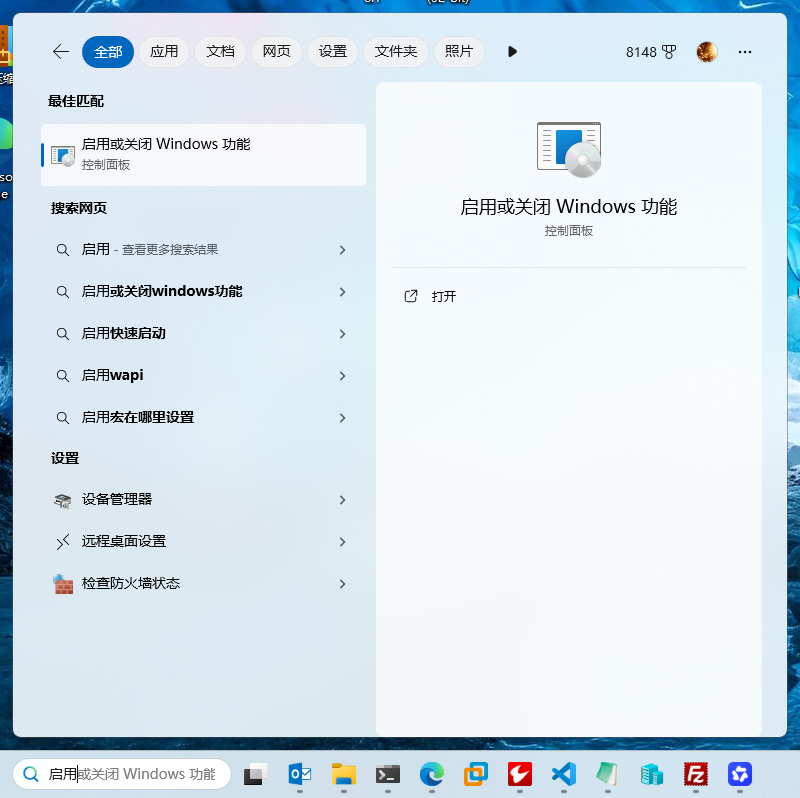
\includegraphics[width=0.6\linewidth]{img/install/start.png}
    \caption{搜索"启用或关闭Windows功能"}\label{fig:start}
\end{figure}
\begin{figure}[H]
    \centering
    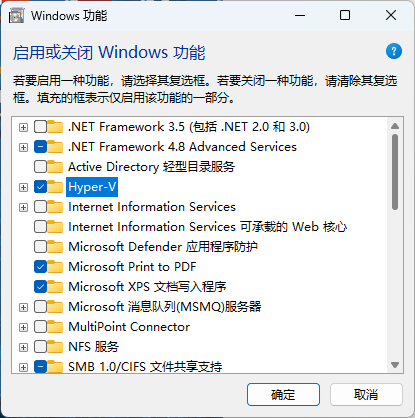
\includegraphics[width=0.4\linewidth]{img/install/hyperv.png}
    \caption{启用Hyper-V}\label{fig:hyperv}
\end{figure}

重启后，在搜索栏输入"hyper-v"，找到"Hyper-V管理器"，打开它。

\begin{figure}[H]
    \centering
    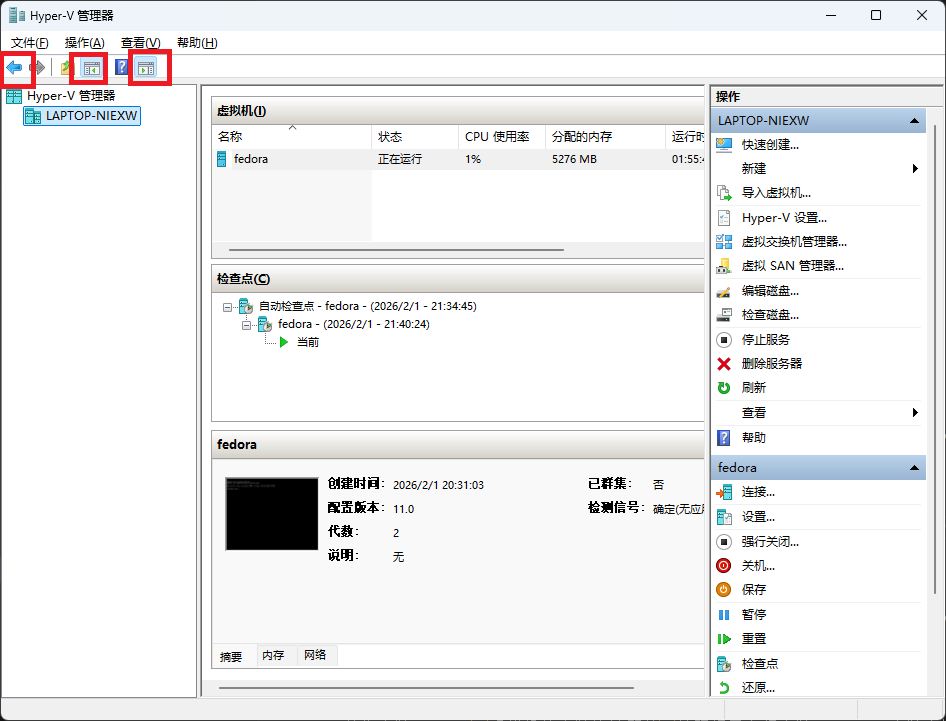
\includegraphics[width=0.8\linewidth]{img/install/hyperv2.png}
    \caption{打开Hyper-V}\label{fig:hyperv2}
\end{figure}

Hyper-V管理器窗口分为三个部分，左边是树型导航窗口，中间是虚拟机列表窗口，右边是虚拟机详细信息窗口。上面的两个小菜单按钮控制左侧和右侧窗片的显示。\emph{有时候，关闭Hyper-V管理器经常会报“未关闭窗口”的错误，可以点击上面最左侧的箭头，将三个窗口全部隐匿，然后再关闭。}

\subsection{安装fedroa}

先去\url{https://fedoraproject.org/server/}下载fedora的iso安装盘，在hyper-v上安装fedora。新建虚拟机，选择fedora的iso光盘，按步骤安装。注意，fedora的硬盘要选得大一些，或者采用Linux卷安装，以便于后期扩展硬盘。

\subsubsection*{替换镜像}

按照\url{https://mirrors.tuna.tsinghua.edu.cn/help/fedora/}的步骤，将fedora的镜像替换为国内镜像。

\begin{lstlisting}[style=bash]
sed -e 's|^metalink=|#metalink=|g' \
    -e 's|^#baseurl=http://download.example/pub/fedora/linux|baseurl=https://mirrors.tuna.tsinghua.edu.cn/fedora|g' \
    -i.bak \
    /etc/yum.repos.d/fedora.repo \
    /etc/yum.repos.d/fedora-updates.repo
\end{lstlisting}

\subsubsection*{配置网络}

Hyper-V默认采用桥接模式，桥接模式下，虚拟机的网络是通过主机的物理网络接口来实现的。建议采用类似VmWare的NAT模式，这样更安全些。但是Hyper-V并不直接支持 NAT模式，需要通过一些配置来实现。

基本思路是在Hyper-V创建一个内部网络，主机配置一个虚拟网卡192.168.200.1/24

\begin{lstlisting}[style=verbose]
New-VMSwitch -Name "vNAT" -SwitchType Internal
New-NetIPAddress -IPAddress 192.168.200.1 -PrefixLength 24 -InterfaceAlias "vEthernet (vNAT)"
New-NetNat -Name "vNATNetwork" -InternalIPInterfaceAddressPrefix 192.168.200.0/24
\end{lstlisting}

然后在Hyper-V上配置fedora的虚拟机，让虚拟机连接到这个vNAT网络，fedora最好配置一个200网段的静态IP，如192.168.200.100/24，可以用nmtui配置。如果没有的话，yum install nmtui安装一下。

\subsection{安装docker}

按照\url{https://docs.docker.com/engine/install/fedora/}步骤安装docker，首先去掉旧版本，用Install using the rpm repository方式安装docker。ps，也可以安装其它Linux操作系统。

\section{导入docker镜像}

\subsection{拷贝源码}

在fedora客户机上建立一个db目录，将db.tar.gz源码拷贝到该目录。实验平台的开发环境是docker，但源码要求放置在guest系统上。

\begin{figure}[H]
    \centering
    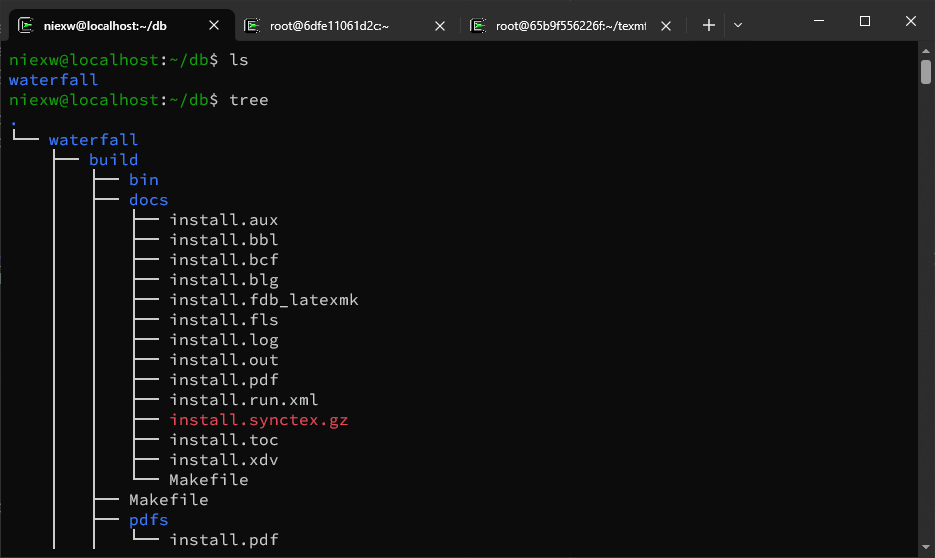
\includegraphics[width=0.8\linewidth]{img/install/source.png}
    \caption{拷贝源码到虚拟机guest系统}\label{fig:source}
\end{figure}

\subsection{导入镜像}

使用import命令导入docker镜像，db.tar为docker镜像。

\begin{lstlisting}[style=bash]
docker import - db < db.tar
\end{lstlisting}

\begin{figure}[H]
    \centering
    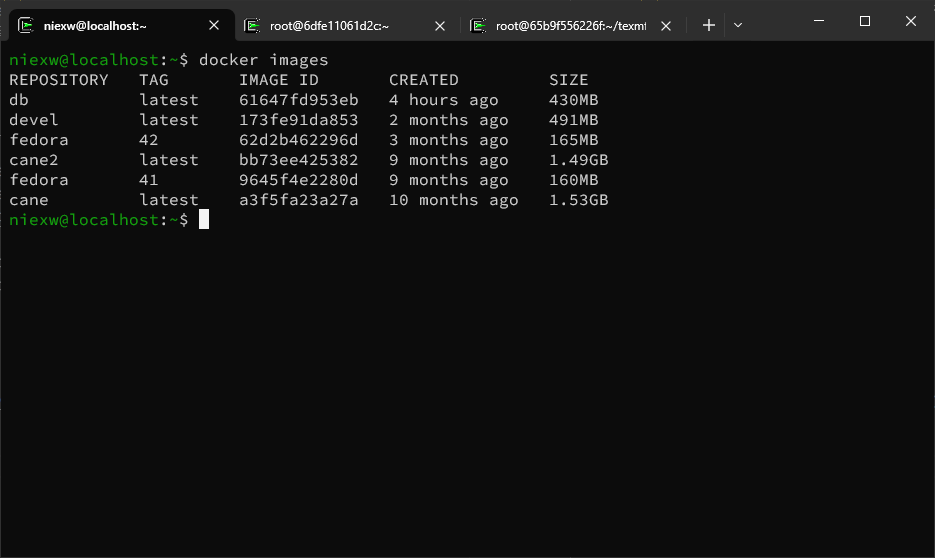
\includegraphics[width=0.8\linewidth]{img/install/docker.png}
    \caption{docker镜像}\label{fig:docker}
\end{figure}

\subsection{启动docker镜像}

使用如下命令启动docker镜像，该命令将docker的22端口映射到fedora虚拟机的10022端口，将fedora系统的/home/niexw/db目录映射到/root/db目录。

\begin{lstlisting}[style=bash]
docker run -d -p 10022:22 -v /home/niexw/db:/root/db --privileged db
\end{lstlisting}

\section{开发工具}

在windows一侧安装shell/vscode等开发工具。

\subsection{连接docker}

可以安装SecureCRT/xShell等工具，然后以10022端口连接docker开发环境。

\begin{figure}[H]
    \centering
    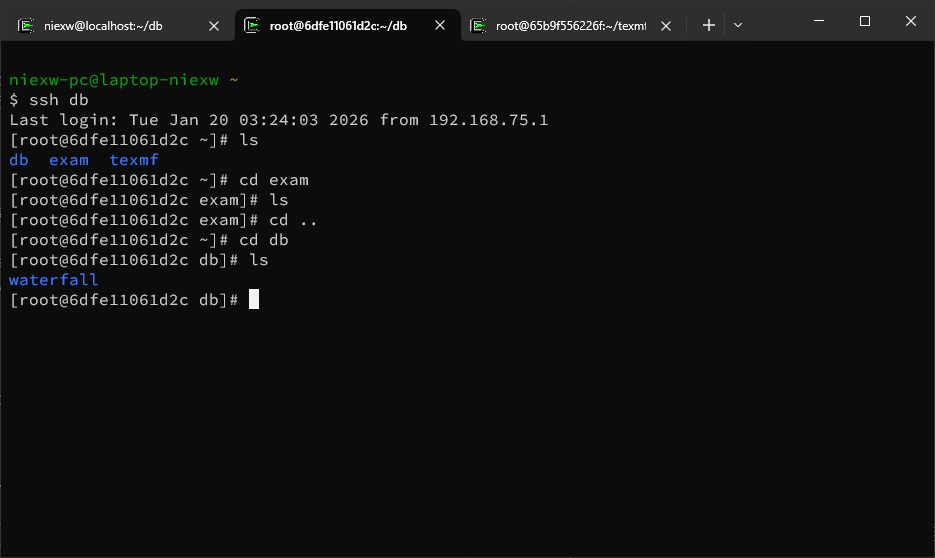
\includegraphics[width=0.8\linewidth]{img/install/ssh.png}
    \caption{使用ssh连接docker}\label{fig:ssh}
\end{figure}

配置系统缺省ssh名字，打开Windows系统当前用户的目录，找到.ssh目录，打开config文件，添加docker的名字。注意，config文件在修改前，需要将文件的安全属性改为可写，改完后再改成勾掉可写选项。

\begin{figure}[H]
    \centering
    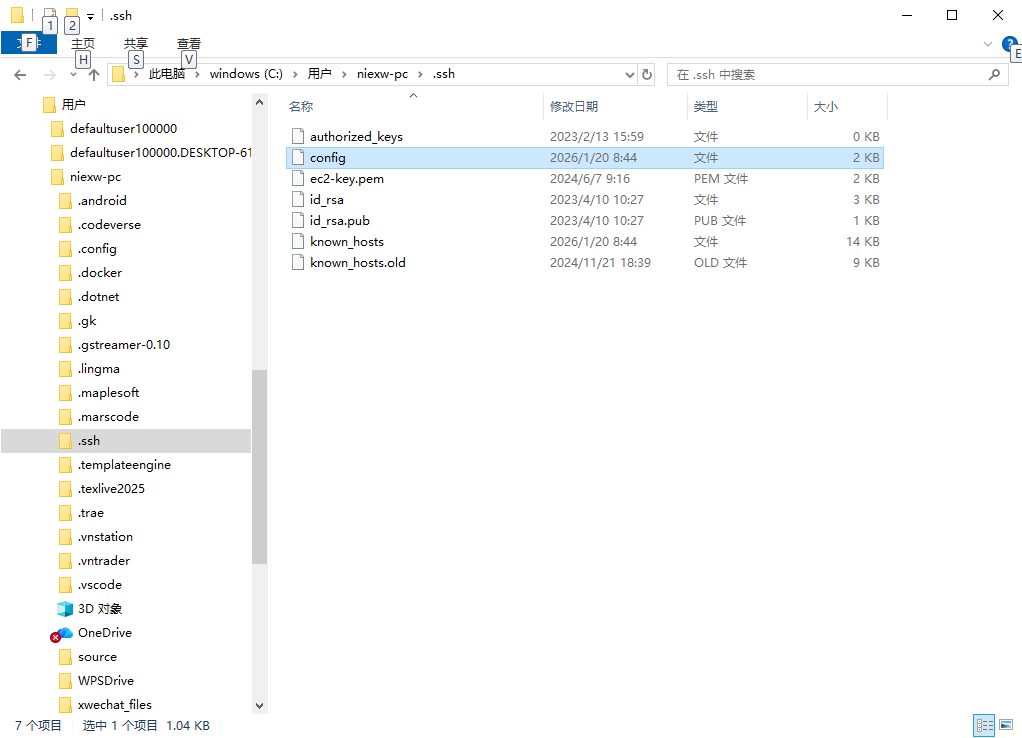
\includegraphics[width=0.8\linewidth]{img/install/config.png}
    \caption{.ssh目录下的config文件}\label{fig:config}
\end{figure}

\begin{lstlisting}[style=verbose]
Host db
    HostName 192.168.75.232
    User root
    Port 10022
\end{lstlisting}

\subsection{vscode}

在Windows上安装vscode，然后点击vscode左下角Open a Remove Window打开远端docker。再用File$\rightarrow$Open Workspace From File菜单打开docker中.vscode-server/db.code-workspace的工作空间。

\begin{figure}[H]
    \centering
    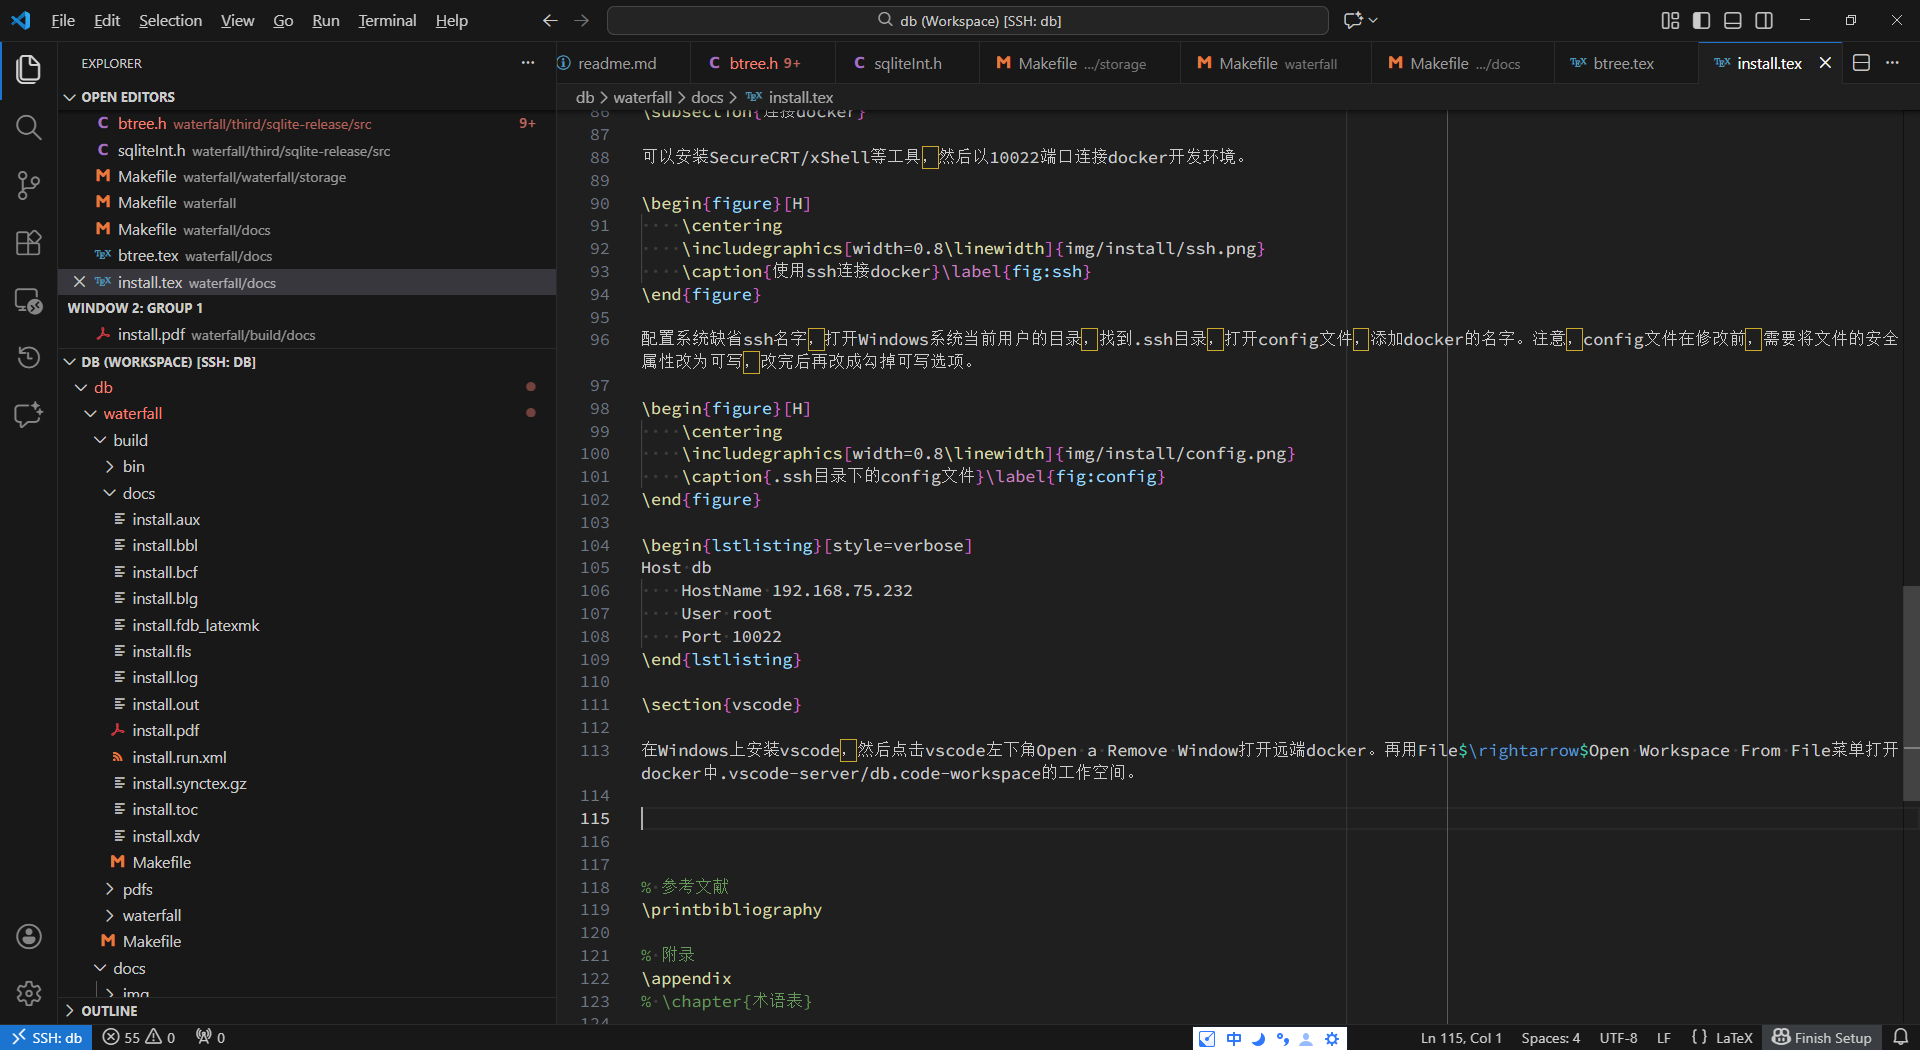
\includegraphics[width=\linewidth]{img/install/vscode.png}
    \caption{使用vscode开发}\label{fig:vscode}
\end{figure}

\section{项目代码}

vscode通过ssh连接docker后，在vscode中建立一个workspace，作为工程项目。

\subsection{目录组织}

代码采用Makefile组织，主要目录如下：

\begin{itemize}
    \item waterfall：项目源码
    \item third：三方库
    \item docs：文档目录
    \item rules：makefile规则
    \item build：编译目录
\end{itemize}

\begin{figure}[H]
    \centering
    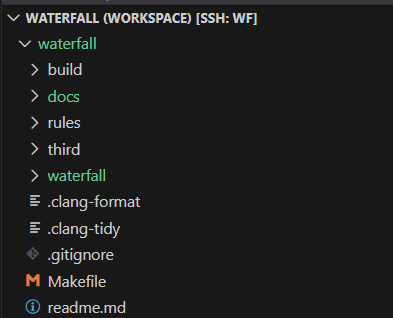
\includegraphics[width=0.5\linewidth]{img/install/directory.png}
    \caption{项目目录组织}\label{fig:directory}
\end{figure}


传统的c/c++代码一般将头文件、源代码分开，头文件用于暴露模块的接口。从实践来看，开发人员一般在开始很难区分出哪些接口需要暴露，哪些是内部定义。本项目中，按照模块组织代码，每个模块对应于一个子目录，子目录下包含头文件、源代码、测试代码等。编译时，一个模块会编译成一个静态库，用于链接成最终制品。

\subsection{c++规范}

本项目使用c++20标准，命名不采用大小驼峰方式，而采用下划线分隔的方式，代码格式由clang-format自动格式化。

\subsection{单元测试}

本项目所有源码均要求做单元测试，测试框架采用Google Test。

\section{rules}

rule目录下是Makefile的规则，项目直接使用Makefile组织工程、自动编译、自动单元测试。项目组织中，鼓励按照目录结构组织模块，每个模块对应一个子目录，每个模块编译一个静态库或者动态库。

\subsubsection*{seperate.mk}

项目将编译目录与源码目录分开，避免编译过程中生成的中间文件污染源码。每次新建编译目录，都需在编译目录下执行make命令。

\begin{lstlisting}[style=bash]
make -f ${SOURCE_DIR}/Makefile
\end{lstlisting}

\subsubsection*{subdir.mk}

项目使用Makefile目录递归编译，在Makefile中添加目录方式如下，注意子目录后要添加斜杠：
\begin{lstlisting}[style=make]
# 子目录
SUBDIRS := coir/ examples/
\end{lstlisting}

\subsubsection*{staticlib.mk}

这个规则文件定义了静态库的编译规则，包括编译选项、依赖关系、目标文件等。

\subsubsection*{sharedlib.mk}

这个规则文件定义了动态库的编译规则，包括编译选项、依赖关系、目标文件等。

\subsubsection*{c++.mk}

这个规则文件定义了c++源码的编译规则，包括编译选项、依赖关系、目标文件等。

\subsubsection*{program.mk}

这个规则文件定义了可执行程序的编译规则，包括编译选项、依赖关系、目标文件等。它包含了sharedlib.mk、staticlib.mk、c++.mk等规则文件，Makefile里一般只需包含program.mk即可。

可执行文件链接的库分为本地库和系统库，本地库、可执行文件都放在build/bin目录下。将本地库与系统库分开，是因为本地可执行程序、单元测试程序往往依赖于本地库，本地库更新这些文件需要重新编译。
\begin{lstlisting}[style=make]
test_uring_SOURCES := test_uring.cc
test_uring_LOCAL_LIBS := -lio -lutils
test_uring_SYSTEM_LIBS := -luring
\end{lstlisting}

所有单元测试代码以test\_开头，直接放在当前源码目录中。单元测试的可执行程序没有放在build/bin目录下，而是放在了build对应的源码目录下。

\subsubsection*{latex.mk}

项目文档使用latex编写，文档目录为docs，latex.mk定义了latex文档的编译规则。docs目录下的doc.sty是文档的样式文件，定义了文档的格式、字体、颜色等，字体安装在fedora docker的/usr/share/fonts/目录下。


% 参考文献
\printbibliography

% 附录
\appendix
% \chapter{术语表}

\end{document}
